\chapter{Implementation of spatial tournaments}
\label{chap:Three}

\section{Introduction}
In this chapter we will discuss the source code committed to the
Axelrod-Python library to implement spatial topology. In addition, some
% I think the main emphasis of this chapter is now these initial results, it
% might be worth making more of the contribution though... Something to think
% about...
initial experiments and results will be discussed. These experiments will be
performed using three chosen topologies and two different sizes of tournaments.

\subsection{Code Discussion}

As analyzed in \autoref{chap:Two}, the Axelrod library uses a
\texttt{Tournament} class to run any given tournament. The \texttt{Tournament}
class itself calls upon another class the \texttt{Match Generator} which is
responsible for generating matches.
In the case of a standard round robin, there is a \texttt{RoundRobinTournament} class
and a \texttt{RoundRobinMatches} class that generates matche parameters for each 2 player
tuple. The parameters and the indices of the pair are used
by the \texttt{build\_single\_match} method. A generator that lives within the
match generator class.
For a round robin tournament the structure of the code is illustrated in~\ref{fig:rbr}.
% Use more verbose labels than rbr (when you're rereading this it'll be
% confusing

\begin{figure}
\centering
    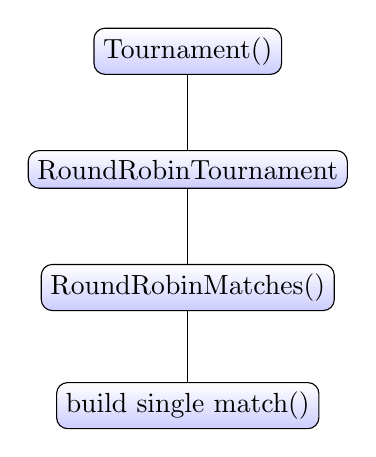
\begin{tikzpicture}[sibling distance=10em,
      every node/.style = {shape=rectangle, rounded corners,
        draw, align=center,
        top color=white, bottom color=blue!20}]]
      \node {Tournament()}
        child { node {RoundRobinTournament}
          child { node {RoundRobinMatches()}
            child { node {build single match()} } }
           };
    \end{tikzpicture}
  \caption{Code structure for a Round Robin tournament.}
  \label{fig:rbr}
\end{figure}

In order for to implement a Spatial topology tournament a similar approach is
needed. Firstly a new \texttt{Match Generator} class was written.  The
\texttt{SpatialMatches} is a class that generates spatially-structured matches.
In these matches, players interact only with their neighbors rather than the
entire population. According to \cite{Archdeacon1996} graphs can be represented
in many different ways, one of which is by lists of edges.  Due to a various
number of python packages that are used for graph manipulation, we want to keep
a more generalized representation of the edges. Thus they will be passed as a
list argument and \texttt{SpatialMatches} will only create matches between the
ending nodes of these edges. Finally the class \texttt{SpatialTournament} runs
the spatial tournament. A representation of the code structure now, that the
spatial tournaments have been added, can be seen in Figure~\ref{fig:cds}

\begin{figure}
\centering
    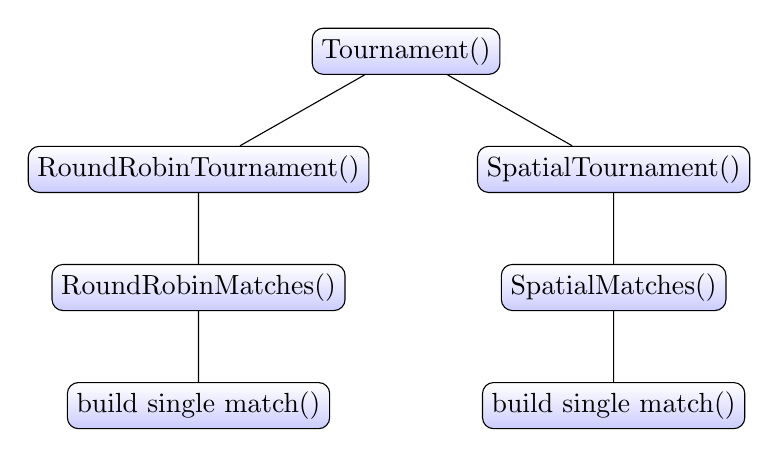
\begin{tikzpicture}[sibling distance=15em,
      every node/.style = {shape=rectangle, rounded corners,
        draw, align=center,
        top color=white, bottom color=blue!20}]]
      \node {Tournament()}
        child { node {RoundRobinTournament()}
          child { node {RoundRobinMatches()}
            child { node {build single match()} } }}
        child { node {SpatialTournament()}
          child { node {SpatialMatches()}
            child { node {build single match()} } }
           };
    \end{tikzpicture}
  \caption{Code structure for when Round Robin and Spatial tournaments are
           implemented.}
  \label{fig:cds}
\end{figure}

In Axelrod library all the components are automatically tested using a
combination of unit, property and integration tests (using \url{travis-ci.org}).
Once a new feature is added to the library, corresponding test must also be written.
The test are used to ensure compatibility and ensure that we get the expected
results. The tests for the \texttt{SpatialTournament} can be found here :
\url{https://github.com/Axelrod-Python/Axelrod/blob/master/axelrod/tests/unit/test_tournament.py}
%: No include them in the text here. Explain what unittesting is. Geraint might
%have some helpful references for this.
under the class \texttt{TestSpatialTournament}.

% Mention version control and discuss what that is as a technique for software
% development.

% Explain that the code was peer reviewed. Get some screenshots of comments from
% Marc and Owen.

% Cite the Axelrod paper and show how your contribution has amongst other things
% resulted in a publication.

% Introduce the next section (just a sentence).

\subsection{Experiment and the three topologies}

% Throughout the English needs a lot of work. Read over it again and again. I
% will fix and point out what I can but I won't have time to fix everything and
% I also want to concentrate on the science.

In this chapter three simple spatial topologies are considered, all with
deterministic neighbourhood size. These will be used to begin to understand how
topology can affect the outcome of tournaments
and which strategies tend to perform well. The three topologies considered are
well represented in the literature \cite{?}:

\begin{itemize}
    \item A cyclic network: the neighbourhood size is 2. % include specific references
    \item A periodic lattice: the neighbourhood size is 4. % include specific references
    \item A complete graph: the neighbourhood size if \(N-1\) (where \(N\) is
        the number of total strategies. This corresponds to a round robin
        tournament. % References
\end{itemize}

In a cycle or circular network consist of a single cycle. It has
equal number of edges and nodes, and each node has degree 2. In~\cite{Szabo2007}
Szabo et all stated that "For spatial models the fixed interaction network is
defined by the sites of a lattice and the edges between those pair whose distance
does not exceed a given value."  The most frequently used structure, and the one
used in this experiment, is the square lattice with von Neumann neighborhood.
Also the most common topology used, again based on literature, is that of a
round robin. A round round topology is nothing else but a complete
graph were every pair of distinct node is connected by a unique edge.
Figure~\ref{fig:networks}, shows an example of all the aforementioned topologies.
Round robin will be mainly used for comparison reasons.
% The English needs a lot of work in the above paragraph. I also think it could
% be condensed in to my bullet points.

\begin{figure}[!hbtp]  % Have a read of http://drvinceknight.blogspot.co.uk/2013/12/explaining-floats-in-latex.html
\centering
    \begin{subfigure}[t]{0.45\textwidth}
    \centering
        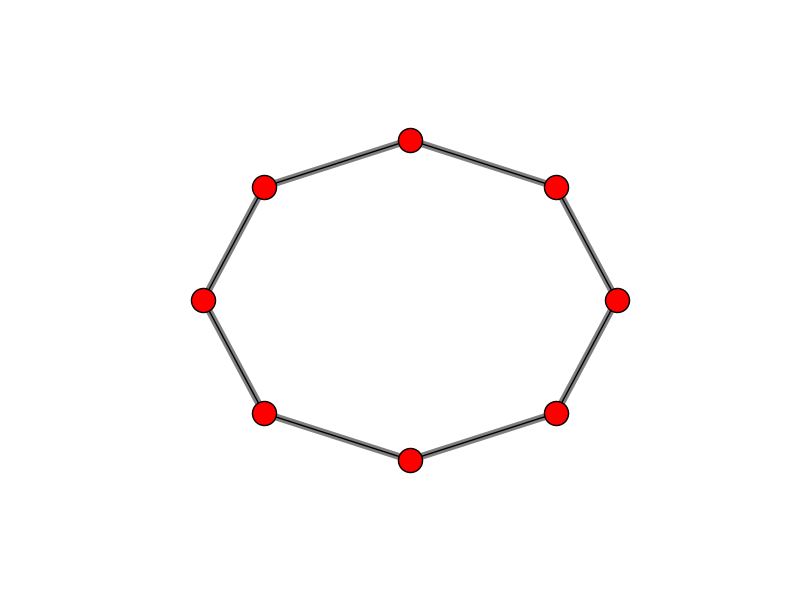
\includegraphics[width=\linewidth]{cycle_network.png}
    \caption{Cycle network.}
    \end{subfigure}
\hfill
    \begin{subfigure}[t]{0.52\textwidth}\centering
    \centering
        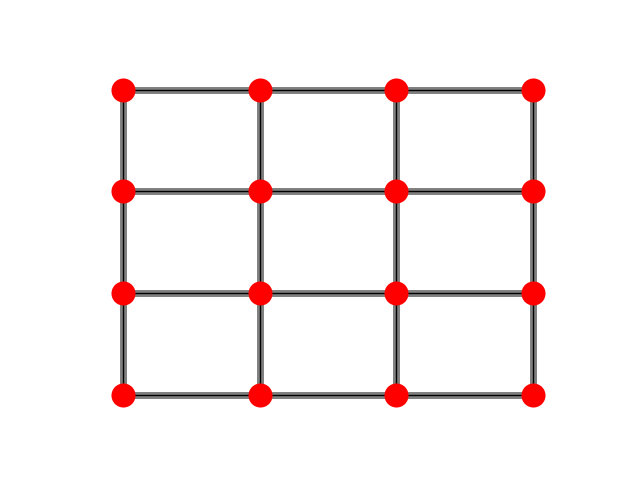
\includegraphics[width=\linewidth]{lattice_network.png}
    \caption{Square lattice with degree 4 network.}
    \end{subfigure}
\hfill
    \begin{subfigure}[t]{0.52\textwidth}\centering
    \centering
        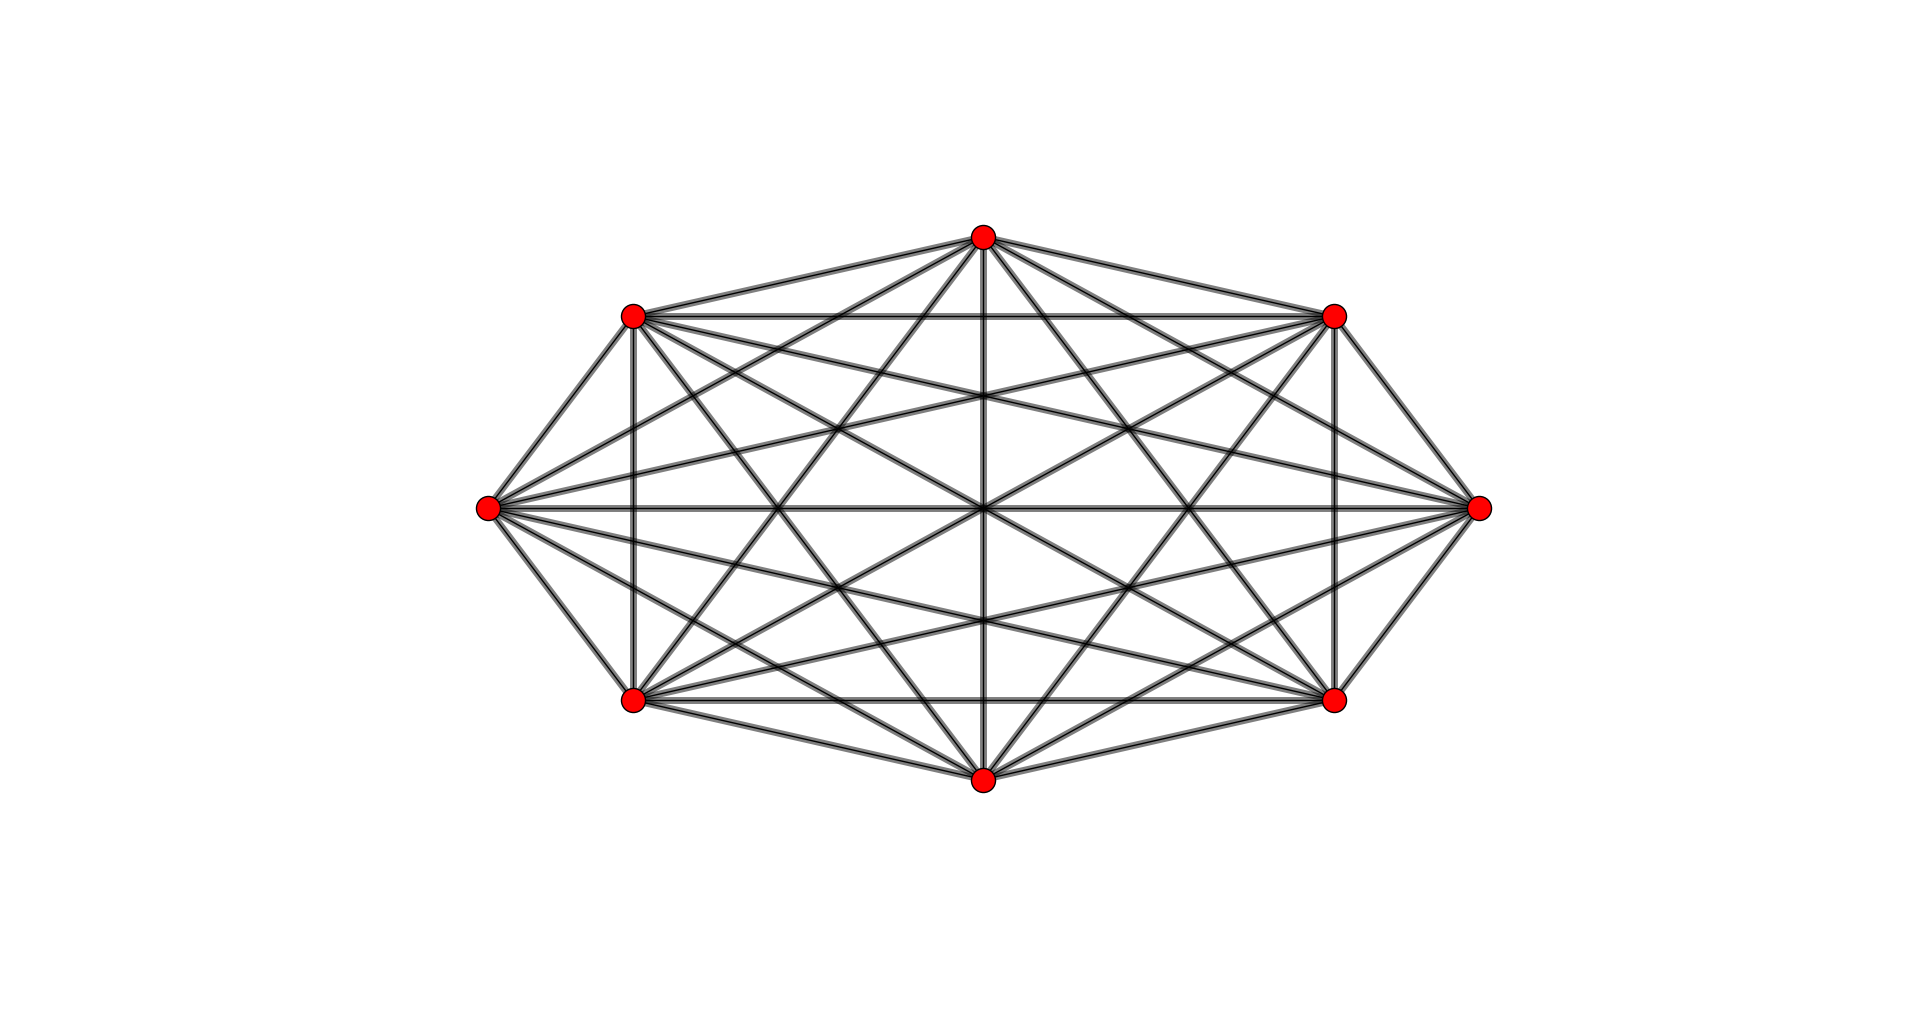
\includegraphics[width=\linewidth]{complete-network.png}
    \caption{A complete or round robin network.}
    \end{subfigure}
\caption{Network topologies.}
\label{fig:networks}
\end{figure}

Thus, we will be performing our experiment with three different topologies, that
of a cycle, a lattice and a complete graph.
% Try and avoid 'we', 'I'. So this sentence would become: The experiments are
% performed on three different topologies: a cycle, a lattice and a complete
% graph. BUT in the particular case it's repeating what was said above so
% perhaps just lose this sentence.
% I'm going to ignore those for the rest of this so read through it all again
% and try and reword.
For each topology, a fixed size of strategies out of the 132 of Axelrod-Python
library are chosen randomly. These strategies create a neighborhood.
The size of these neighborhoods will range. Let \( s\) be the size of
% This isn't quite correct: we talk about a neighbourhood of node, here you're
% taking about the whole set of nodes.
the neighborhood, where \(s \textrm{ }\{ s=5 \textrm{ and } s=50 \}\).
% There is no need for this shorthand notation. I would get rid of \(s\). If you
% wanted to you could talk about \(S_t\) as the set of strategies for a given
% random tournament and then the size would be \(|S_t|\) but I'm not sure that's
% necessary.
Subsequently, the strategies are allocated on the graph, based
on the topology, and they compete with their neighbors on a IPD tournament.
For the cyclic and lattice topology, once the first game is complete,
the strategies are randomly shuffled and allocated on the graph again. This aims
to ensure that their particular position on the network is taken in to account.
Another tournament is performed this time with different neighbors of a
neighborhood interacting.
% I do not know what this sentence is trying to say.
This is repeated 10 times.
The selection of strategies and creation of neighborhoods is repeated 100 times
and each tournament of an IPD consists of 200 turns and 10 repetitions.
% I think you should draw a picture of this or perhaps write some pseudo code
% (kind of like the things we've been writing on my whiteboard):
% http://tex.stackexchange.com/questions/163768/write-pseudo-code-in-latex

By setting an axelrod-seed~\footnote{A function used by the library, which sets
both seeds for Numpy and the standard library.In general, seeds allow us
reproduce the same players and tournaments.}, the 100 neighborhoods for the
topologies are the same, of course their allocation to the graphs differs because
of the random shuffle.
% You're going in to to many details here: the reader could potentially have no
% idea what Numpy is. If you write this out with pseudo code you can simply say
% that you're looping over seeds and then include some nice reference/comment
% about why you're doing that.

For the experiments to run we have created three simple scripts, one for every
given topology. This code allow us to generate random
neighborhoods and pass them as nodes on their respective graphs. The tournaments
then are played and produce results.
% The above should be replaced by saying that you're running this on a
% supercomputer. The fact that they are scripts is not important, and the other
% details have been said before.

We want to keep track of some given
parameters and to achieve that, the pandas python library is used. We create
a data frame and it allow us to pass all the new values of the parameters that
are produce and afterwards export it to a csv file. Some parameters needed for our
analysis were not given by the Axelrod-Python library, thus a few simple
functions for neighbors and their score were also written.
% The English needs to be fixed here. I think you can have a general paragraph
% about libraries used for data preparation and analysis: pandas, jupyter and
% matplotlib used for analysis and networkx used to generate networks.

The Axelrod tournaments themselves make usage of match memory and CPU power and
by adding
these additional rules to the tournaments was only increasing in usage. For that
reason all the tournaments and their results we are run in Raven. Raven is the
master computer of Cardiff University. All the scripts and pbs file, for
communicating with Raven, can be found in my personal GitHub account
\url{https://github.com/Nikoleta-v3}.
% Yup this is good, see my previous comment. Also: not 'my personal...', can be
% found on github at <url>.


% I have to create a repository with all the files for the dissertation and clean
% thing up a little bit. Then I will add the new link here. and a message 'Like my page :D'

% Haha: good idea :) We'll also talk about using something like zenodo.org to
% 'freeze' your data. We should talk about this.

% Introduce the next section but also map out what is in each coming section:
% "In the next section we will ... before in Sections blablbla doing
% blablabla... and finally summarising and offering further avenues of research
% in Section blablabla

\subsection{Initial Analysis}

For each of the tournament run, the following parameters are recorded:

\begin{itemize}
    \item List them all here: bullet points will be easier to read.
\end{itemize}

This section will describe the findings of a basic statistical analysis of these
records.

For the spatial tournaments, for both neighborhood sizes (5 and 50)
% Not neighbourood sizes: tournament sizes. Also, we have so far used the
% terminology that the complete graph is a spatial tournament (just a boring
% topology so this needs to be reworded to fit with that).
we achieved 1000 tournaments. Containing 100 different strategy sets, where each
the exists for 10 tournaments.

Moreover, for the cycle experiment we can see in Table~\ref{sum-cicle}, that degree is
fixed at 2 and the payoffs are fixed to \(R=3, P=1, S=0, T=5\) for both
\( s=5\textrm{ and } s=50 \). For tournaments of size 5, the mean average score
% Don't like s, there is no need for it (you're not carrying out algebraic
% manipulations with it). Fix this throughout.
is 2.45, with a minimum value of 0.0175 and a maximum value of 4.95. The
mean average score of the neighbors score is 980.95 with a standard deviation
of 219.87. Moreover the minimum value is set at 141.55 and the maximum at
1756.50. The mean average score does not seem to differ for \(s=5\),
which is at 2.39. Though, in the experiment with a size of fifty a strategy
achieved a score of 0. Additionally the average score of the neighbors ranges
from 19.30 to 1884.5. In both cases of size the clustering coefficient is zero
and the connectivity due to fixed degree is 2.
% and the connectivity?... (something missing here, do you mean the clustering
% coefficient and the connectivity are 0 as the degree is fixed?
% Also I forget, but assuming you have described what these things mean in C2,
% you should remind the reader and just point them to C2.

% This table looks good BUT (IMPORTANT) Read these (and then improve all your
% tables)
% - http://www.howtotex.com/packages/improve-your-tables-with-booktabs/
% - https://www.inf.ethz.ch/personal/markusp/teaching/guides/guide-tables.pdf
%   (particularly the before and after slide)
\begin{table}[!hbtp]
\centering
\begin{adjustbox}{width=1\textwidth}
\small
\begin{tabular}{@{}|l|l|l|l|l|l|l|l|l|l|@{}}
\toprule
Cycle & \multicolumn{3}{c}{s=5 and s=50}  & \multicolumn{3}{c}{s=5}                              & \multicolumn{3}{c}{s=50}                             \\\midrule
% No s
       & (R,P,S,T) & degree & connectivity & average score & average neighbors score & clustering & average score & average neighbors score & clustering \\\midrule
mean   & (3,1,0,5) & 2.0    & 2.0          & 2.456690      & 980.952580              & 0.00       & 2.394577      & 957.238664              & 0.00       \\\midrule
std    & (0,0,0,0) & 0.0    & 0.0          & 0.748772      & 219.875803              & 0.00       & 0.777189      & 231.321350              & 0.00       \\\midrule
min    & (3,1,0,5) & 2.0    & 2.0          & 0.017500      & 141.550000              & 0.00       & 0.000000      & 19.300000               & 0.00       \\\midrule
max    & (3,1,0,5) & 2.0    & 2.0          & 4.950000      & 1756.500000             & 0.00       & 5.000000      & 1884.500000             & 0.00       \\ \bottomrule
\end{tabular}
\end{adjustbox}
\caption{Summary table for topology circle.}
\label{sum-cicle}
\end{table}
% No nee for this level of precision (use less decimal places, 2 or 3 are
% sufficient.

For the lattice topologies a table that summarizes the data set is shown in Table
~\ref{sum-lattice}. For both size values the payoffs are the same (\(R=3, P=1, S=0, T=5\))
and the degree is fixed at 4. For \(s=50\) the mean average score
% No s (just commenting to remind you: find them all).
varies between 0.018 and 4.97. The average score of the neighbors varies between
832.67 and 2895.42. Much higher than both the cycle experiments achieved. This
is understood to be
based on the fact that the number of neighbors is now doubled. For \(s=5\)
the mean score is 0.57 and the mean average neighbor score 2.45.
The clustering coefficient is 1 and for \(s=50\) is 0.5.
This shows that in the lattice example the strategies tend to create groups.
% What do you mean about 'groups'. I don't disagree, just curious.

\begin{table}[!hbtp]
\centering
\begin{adjustbox}{width=1\textwidth}
\small
\begin{tabular}{@{}|l|l|l|l|l|l|l|l|l|l|@{}}
\toprule
Lattice & \multicolumn{3}{c|}{s=5 and s=50} & \multicolumn{3}{c|}{s=5}                             & \multicolumn{3}{c|}{s=50}                            \\ \midrule
       & (R,P,S,T) & degree & connectivity & average score & average neighbors score & clustering & average score & average neighbors score & clustering \\ \midrule
mean   & (3,1,0,5) & 4.0    & 4.0          & 2.450782      & 1958.569220             & 1.0        & 2.393000      & 1912.748200             & 0.5        \\ \midrule
std    & (0,0,0,0) & 0.0    & 0.0          & 0.576812      & 287.638191              & 0.0        & 0.590971      & 268.375436              & 0.00       \\ \midrule
min    & (3,1,0,5) & 4.0    & 4.0          & 0.527500      & 1059.775000             & 1.0        & 0.018750      & 832.675000              & 0.5        \\ \midrule
max    & (3,1,0,5) & 4.0    & 4.0          & 4.245000      & 2518.700000             & 1.0        & 4.973750      & 2895.425000             & 0.5        \\ \bottomrule
\end{tabular}
\end{adjustbox}
\caption{Summary table for the lattice topology.}
\label{sum-lattice}
\end{table}

\newpage

Finally, for the round robin tournaments, 100 tournaments were performed for both
 sizes. Parameters such as neighborhood size and neighbor's score
were not computed for the round robin topology. This is because all players
interact with each other and so we would not get any additional information. In
Table~\ref{sum-rr}, we can see the average score the strategies achieved
in this topology for both sizes. In a tournament of size 50, the mean average
score is 2.39 with a standard deviation of 0.335. For \(s=5\) we can notice that the values
are almost equal to those of the lattice topology with \(s=5\). % So what?
% What's interesting about this?

\begin{table}[H]
\centering
\begin{tabular}{|l|l|l|}
\hline
Round Robin & \multicolumn{1}{c|}{s=5} & \multicolumn{1}{c|}{s=50} \\ \hline
% No s
            & average score            & average score             \\ \hline
mean        & 2.447105                 & 2.393220                  \\ \hline
std         & 0.576014                 & 0.335552                  \\ \hline
min         & 0.527500                 & 1.523673                  \\ \hline
max         & 4.245000                 & 3.339592                  \\ \hline
\end{tabular}
\caption{Summary table for round robin topology.}
\label{sum-rr}
\end{table}

In this section we gone through the structure of the source code for implementing
the Spatial Tournament, by adding to the Axelrod-Python library. Furthermore, now
that the code is usable various experiments were conducted with different topologies
and number of players participating in each tournament. An overview of the
data sets produced was done but now in the following sections we will go though
some more analysis on the results.
% Good paragraph (just get rid of 'we').
% From a language point of view is writing in that form (so not with 'we') more
% difficult? Just asking in case you would like more support. (You'll need to
% write that way anyway).

\newpage
\section{Analyzing the effect of the topologies}
\label{sub:effects}
% No points for short variable names so
% \label{sub:analyzing_the_effect_of_the_topologies} would be fine. Not telling
% you to change it just saying you can use nice long label names to help you
% when you come back to these things.

In the data all 132 strategies of Axelrod-Python library have participated at
least in one tournament. Here we will go through the strategies and their
performance in each experiment. Not all strategies participated in an equal
number of tournaments. Forcing the strategies to perform in a uniform number is
not an option as we want to keep the random effect for validation of the
results. On could argue that by participating in a larger number of tournaments,
the probability of winning increases as well. Thus, for a measure of
performance, instead of using the number of tournaments won, the analysis will
be using the ratio of wins. By wining ratio we mean the number of tournaments a
% The winning ratio is defined as...
strategy got first place divided by the number of tournaments the strategy
competed in. Additionally, the normalized average score each strategy achieved
will also be studied. Mainly to study the variation, helping us to make
conclusions on the performance of a strategy.  Lastly, having all different
factors such as degree, neighbors, clustering, scores etc building a regression
model could point out effects on the results.
% This last part is good (saying what you're going to do) just include some
% pointers to the actual sections.

\subsection{Winning Ratio}
\label{sub:winning-ratio}

The winning rations for all three topologies for tournaments of size 5
are shown in Figure~\ref{fig:winning-five}. In the experiment where the
strategies compete on a cycle 124 strategies out of the 132 have a
winning ration greater than zero. In other words 8 strategies won no
tournaments. These strategies are ALLCorALLD,
Tricky Cooperator, ThueMorseInverse, Hard Tit For 2 Tats, SolutionB5, Cycler DDC,
Prober and BackStabber.
% Put these in a bullet point list or a table with a VERY brief description of
% what they do.
% I'm really surprised that BackStabber won no tournaments...
In the lattice topology as well, 8 strategies do not have
a non-zero winning ratio. Fortress4, Bully, Tricky Cooperator, Hard Go
By Majority: 5, 10 and 40. Also Cycler DDC and ALLCorALLD have a similar
performance in this topology as well.
% Same comment about putting the strategies in a table.
In the round robin tournament various strategies  % How many?
ranked last, among them Fortress4 and the whole family of Hard Go By Majority.
% If the number is not stupid perhaps put them in a table also.

On the other hand the strategies with the highest winning ratio for each
topology are as follows:

\begin{itemize}
  \item Cycle topology with a winning ratio of 0.56 ZD-GEN-2, followed by Punisher
        with 0.55
  \item Lattice topology with a ratio of 0.45 BackStabber and Meta Majority
        Memory one
  \item Round Robin topology with a winning ratio of 1 : Raider, Gradual, Limited
        Retaliate(0.05/20) and BackStabber.
        % See how well Backstabber does here and on the lattice...
        % I wonder what's going on... Interesting...
        % Will be good to get those line plot things.
\end{itemize}

In every topology the highest ranking strategy between the size five experiments
are different. Only BackStabber seems to be repeated, even so in the cyclic topology
 it had a winning ratio of zero. ALLCorALLD, did badly in all
three topologies.

When considering tournaments of size 50
no strategies have a zero ratio (in any topology).
% Give a little explanation for this: why do we think that is? Does this perhaps
% mean we need to run the size 5 strategies more? To get more diversity in the
% strategy sets? What do you think?
Figure~\ref{fig:winning-fifty}, illustrates the ratios
for each topology in ascending order. The strategies with the highest winning ratio
for each respective topologies are as follow :

\begin{itemize}
  \item Cycle topology with a winning ratio of 1.3 Raider
      % Winning ratio of 1.3? 1.3 > 1
  \item Lattice topology with a winning ratio of 1.3 Raider
  \item Round Robin topology with a winning ration of 0.833 EvolvedLookerUp
\end{itemize}

Unexpectedly, strategy Raider seems to have first place in both
the cycle and the lattice topology. It achieved a winning ration of 1.3, 0.5
more than the strategy ranked second. Another surprise in the results is
that of the round robin topology. Where a large number of strategies have a
winning ratio
of zero. Only 14 strategy managed a ratio higher than zero. The strategy with
the highest one of all was EvolvedLookerUp.

Overall, in all six experiments the only strategy that seems to be repeatedly
have a high performance is
Raider. Compared to all the other strategies that outperformed the rest the seem
to be no similarity in their way of structure and play. Here we could use
a characterization to compare the strategies more efficiently. The winning ratio
seems to vary from zero to 1.3 and in the round robin topology many strategies
seem to get zero.
% winning ratio higher than 1?

% add plot
% The line plot yes? I think this will be 3 line plots, one for each comparison
% of topology. This will be very good to have.

\begin{figure}[!hbtp]
\centering
    \begin{subfigure}[t]{1\textwidth}
    \centering
        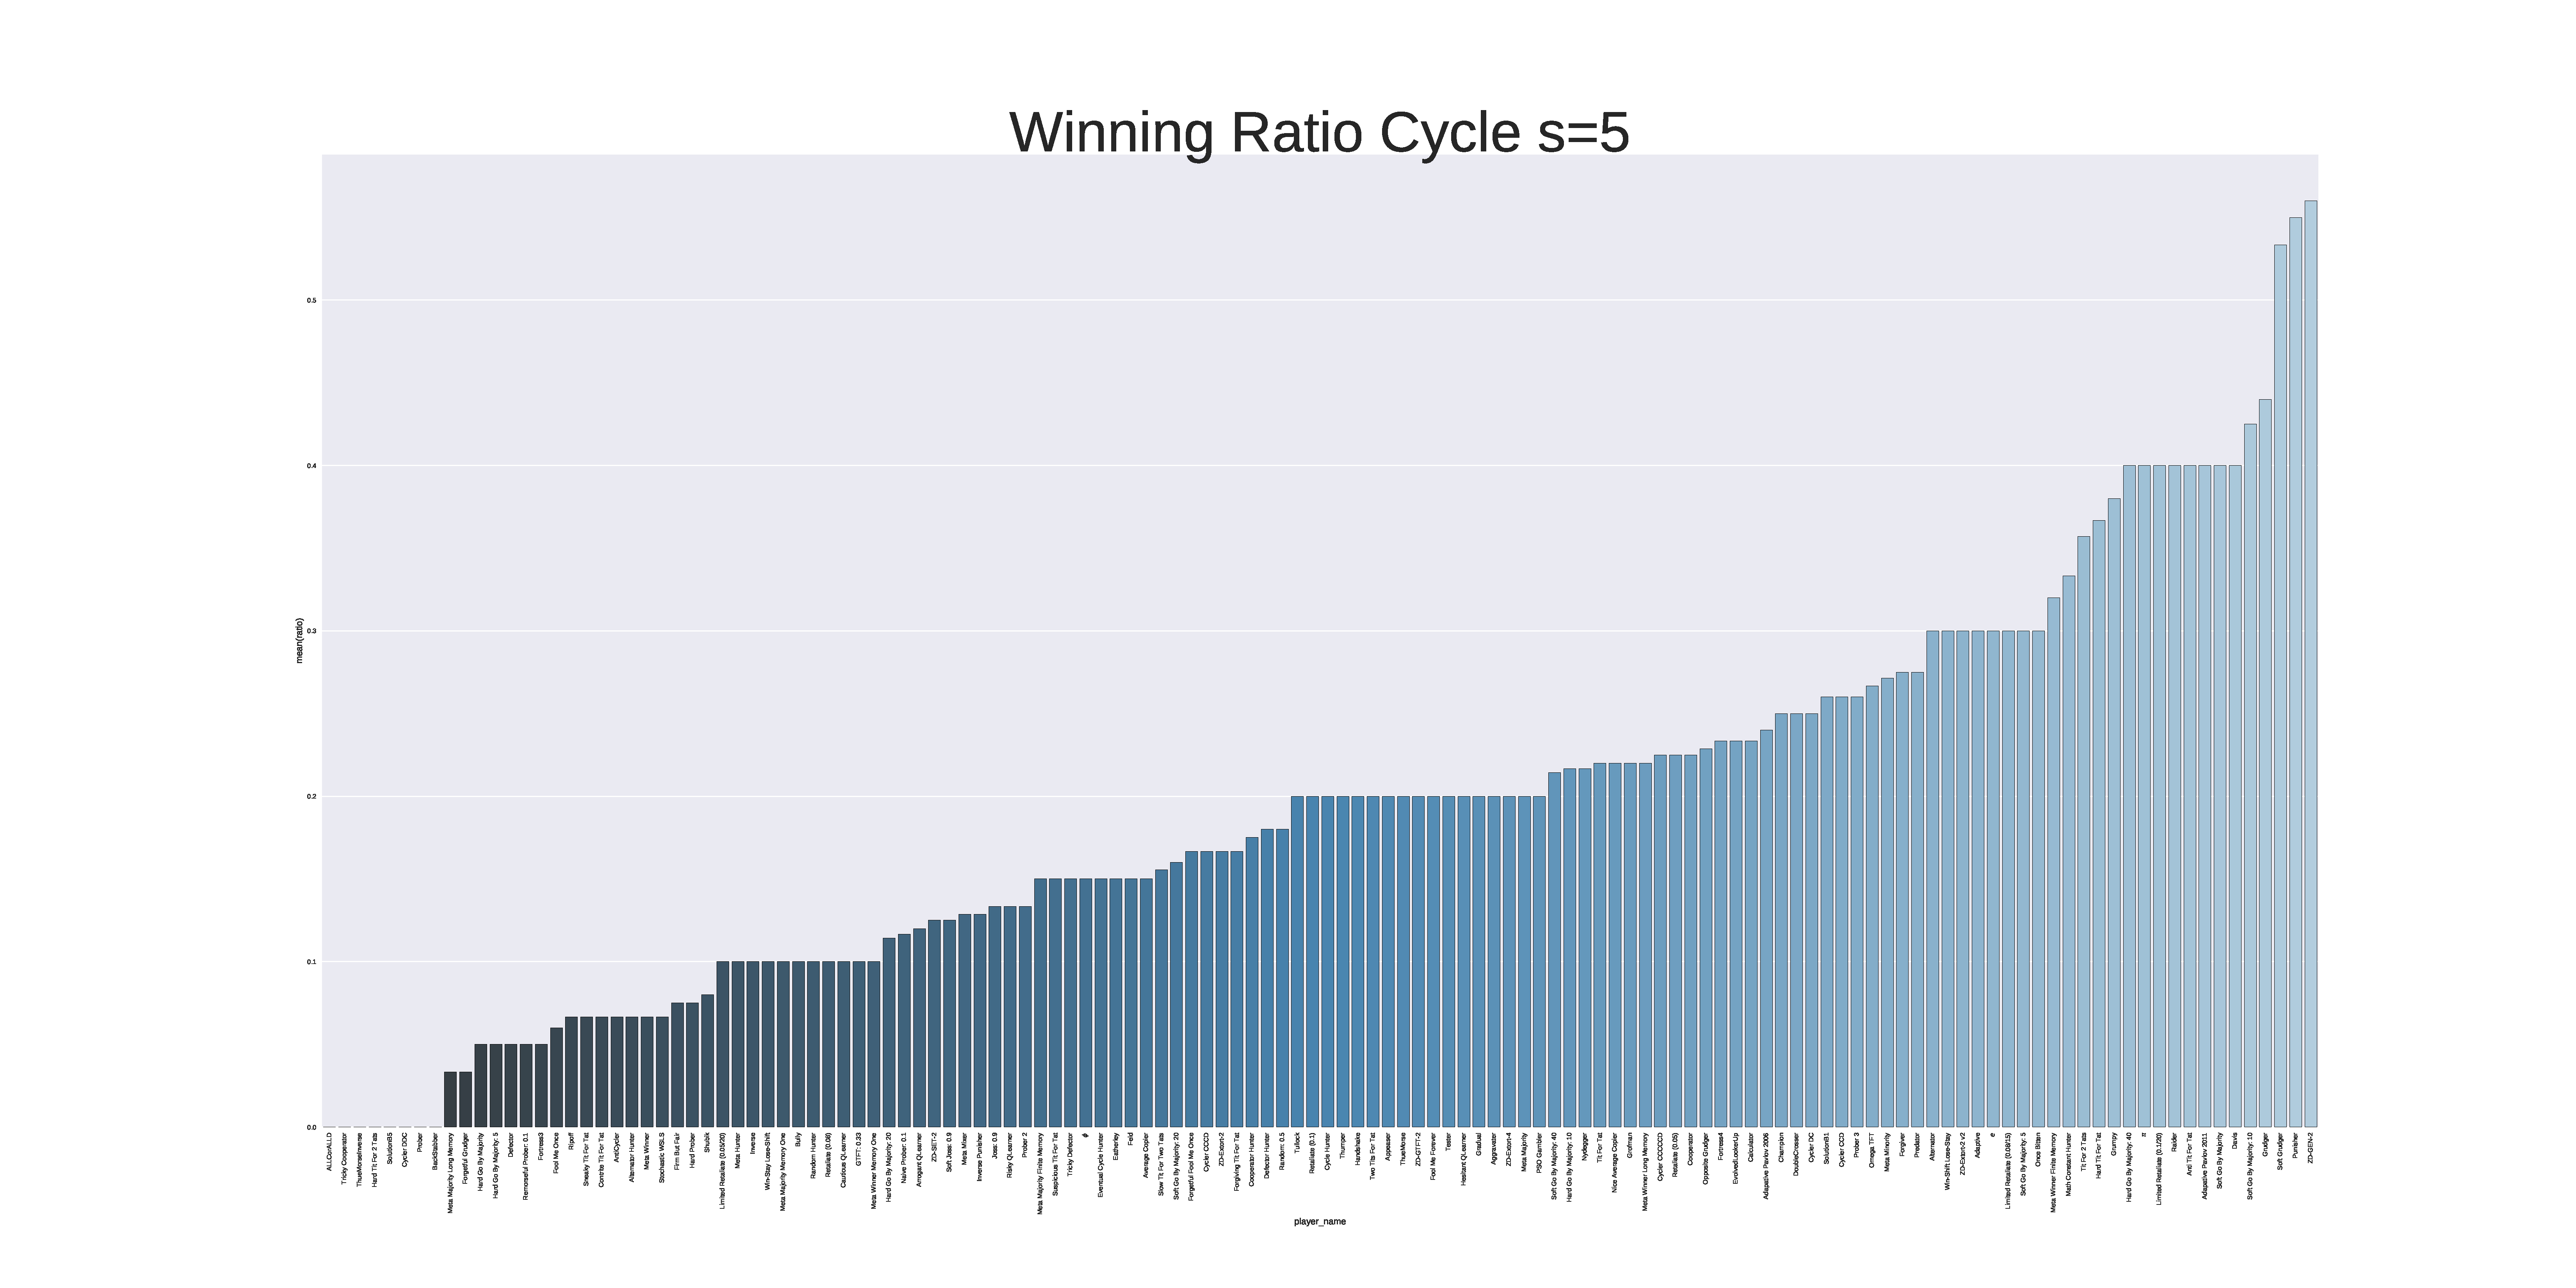
\includegraphics[width=\linewidth]{winners-cycle_five.pdf}
    \caption{Winning ration cycle s=5.}
    \end{subfigure}
\hfill
    \begin{subfigure}[t]{1\textwidth}\centering
    \centering
        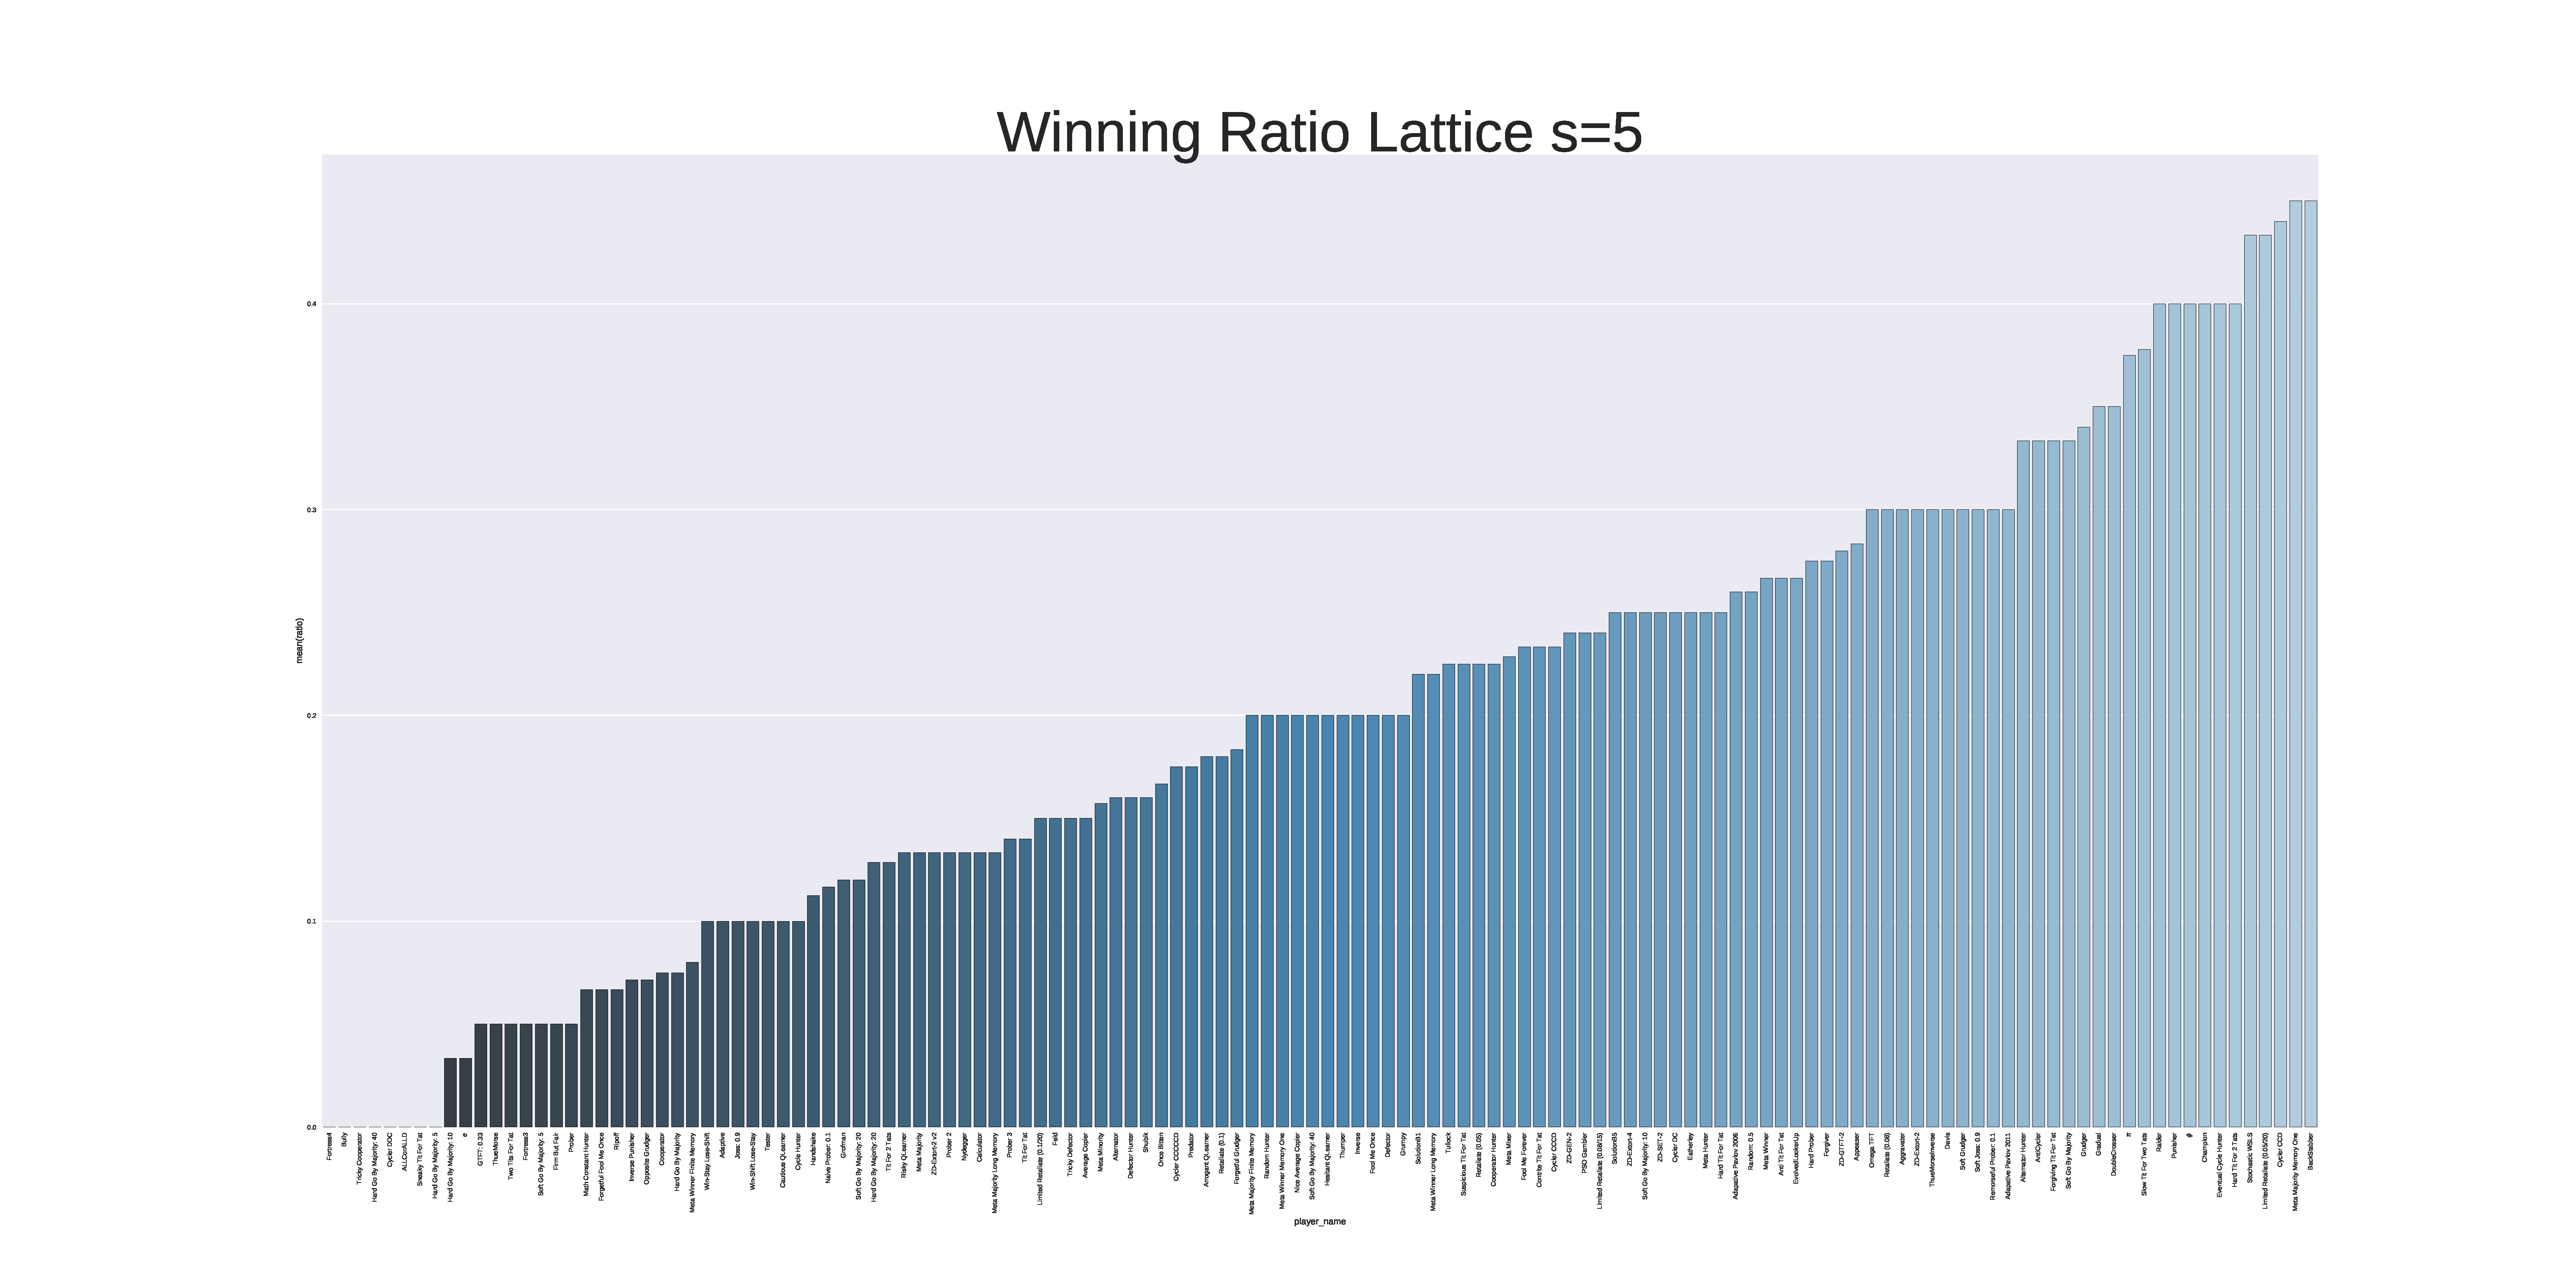
\includegraphics[width=\linewidth]{winners-lattice_five.pdf}
    \caption{Winning ration lattice s=5.}
    \end{subfigure}
\hfill
    \begin{subfigure}[t]{1\textwidth}\centering
    \centering
        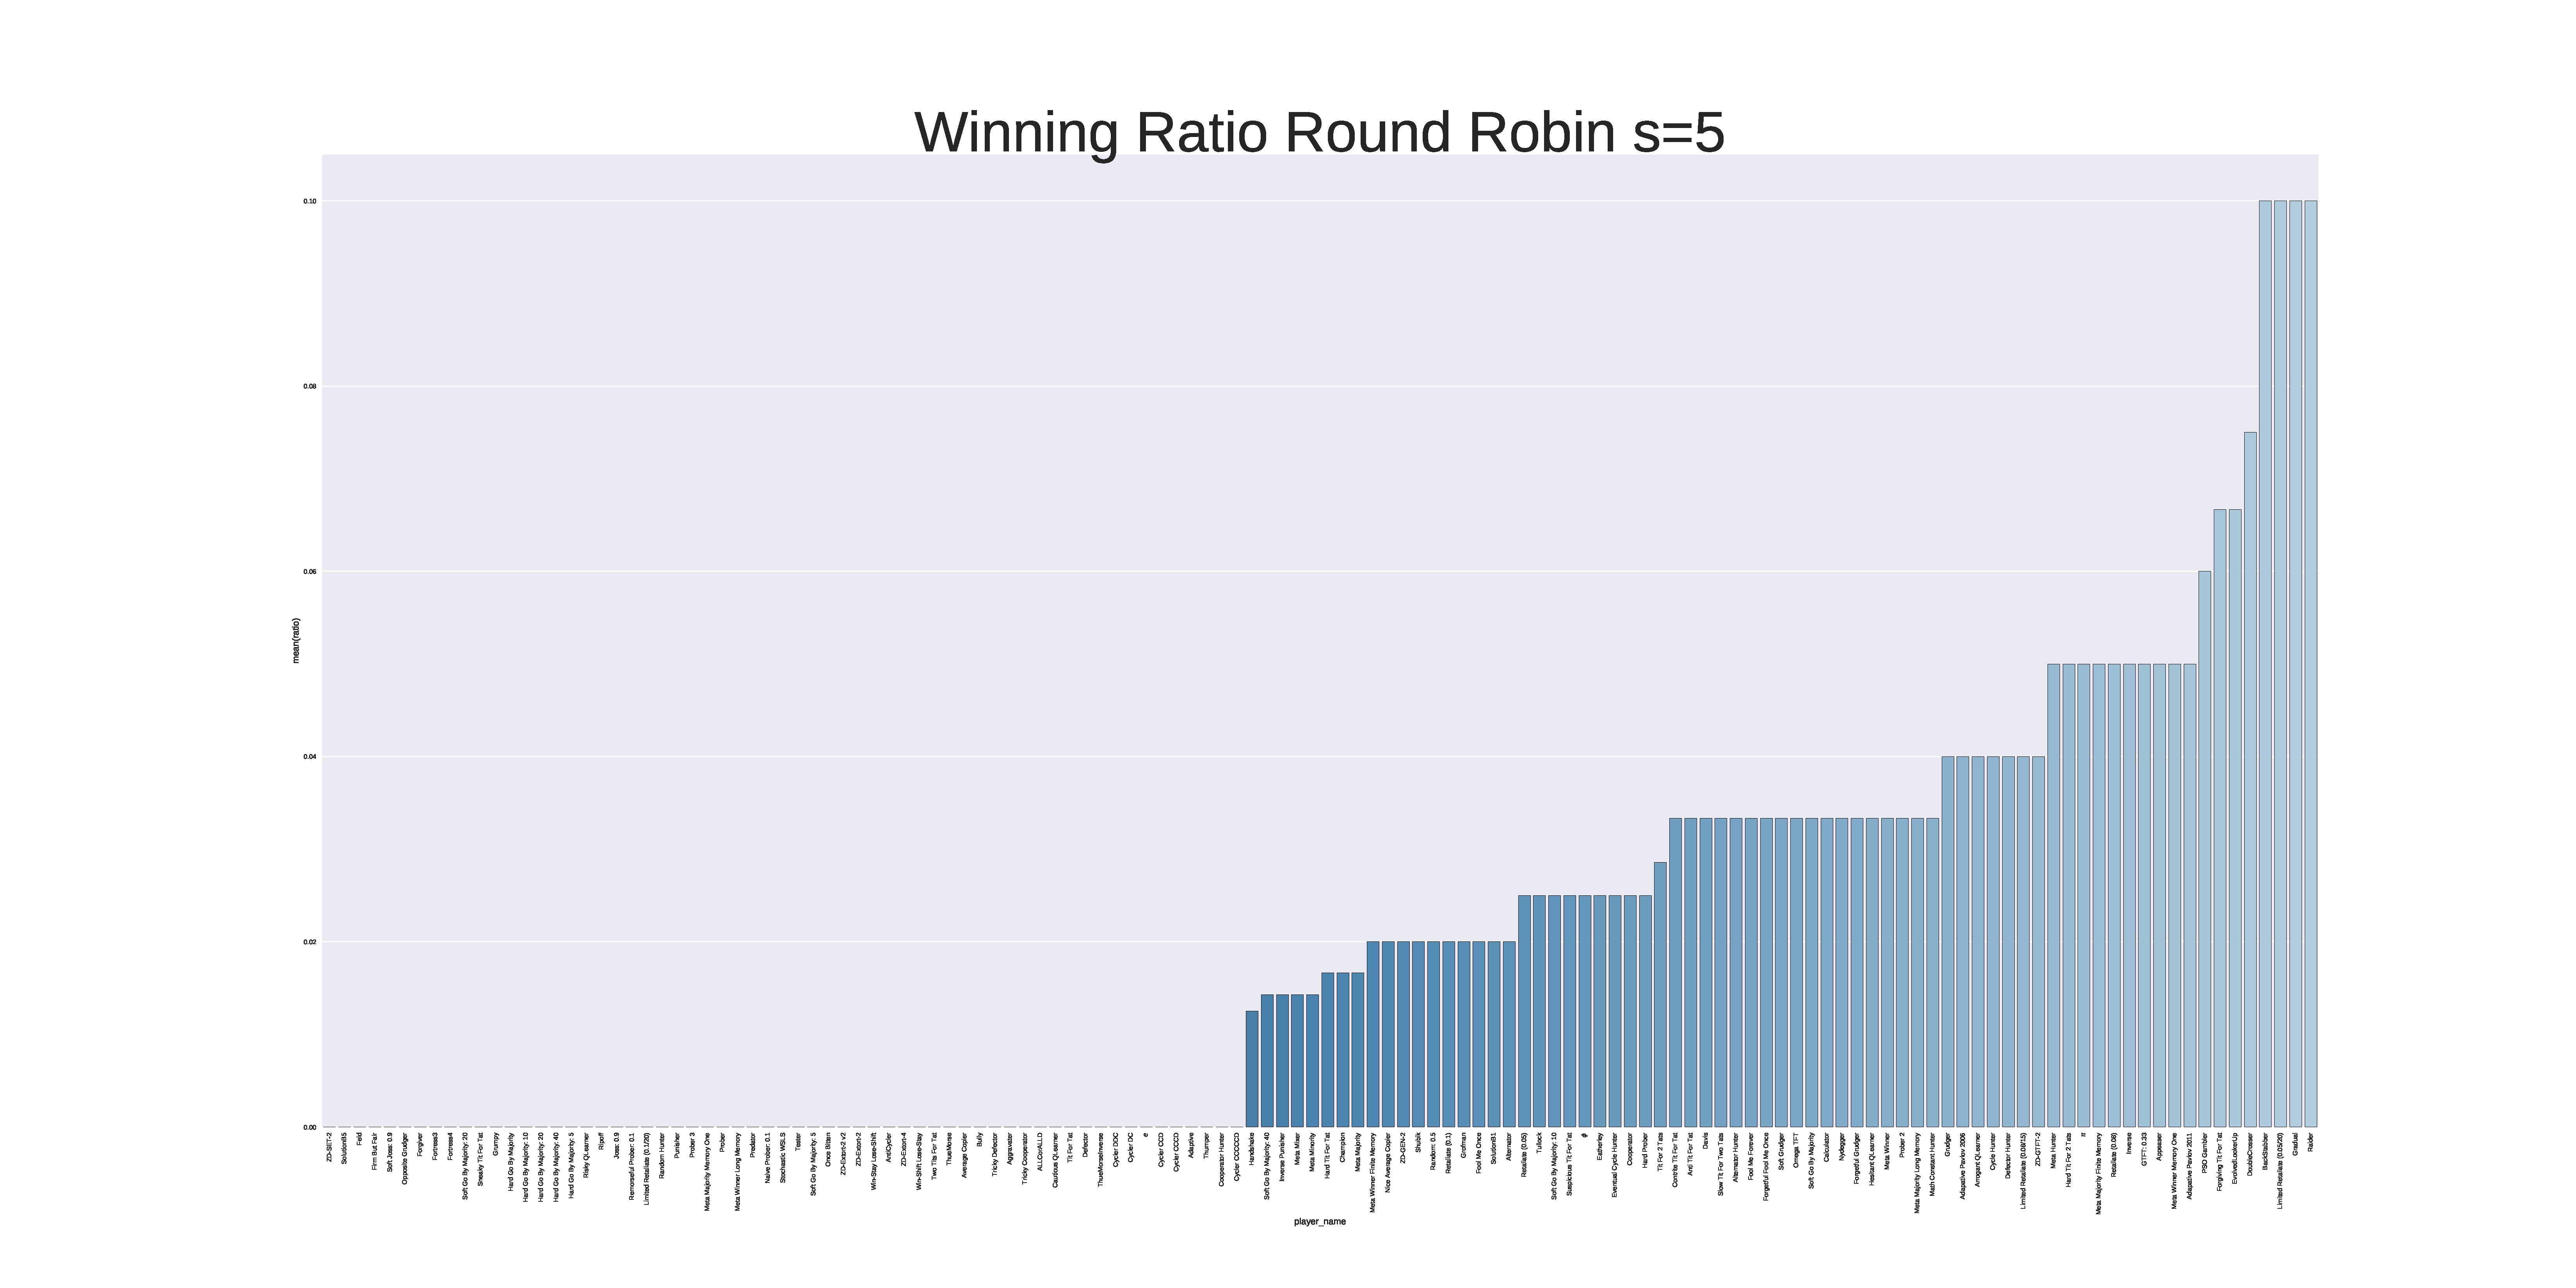
\includegraphics[width=\linewidth]{winners-rr_five.pdf}
    \caption{Winning ration round robin s=5.}
    \end{subfigure}
\caption{Winning ratio for all three topologies s=5.}
\label{fig:winning-five}
% Why are these plots bar plots? Should they just be scatter plots?
% Same comment for all of them.
\end{figure}

\begin{figure}[H]
\centering
    \begin{subfigure}[t]{1\textwidth}
    \centering
        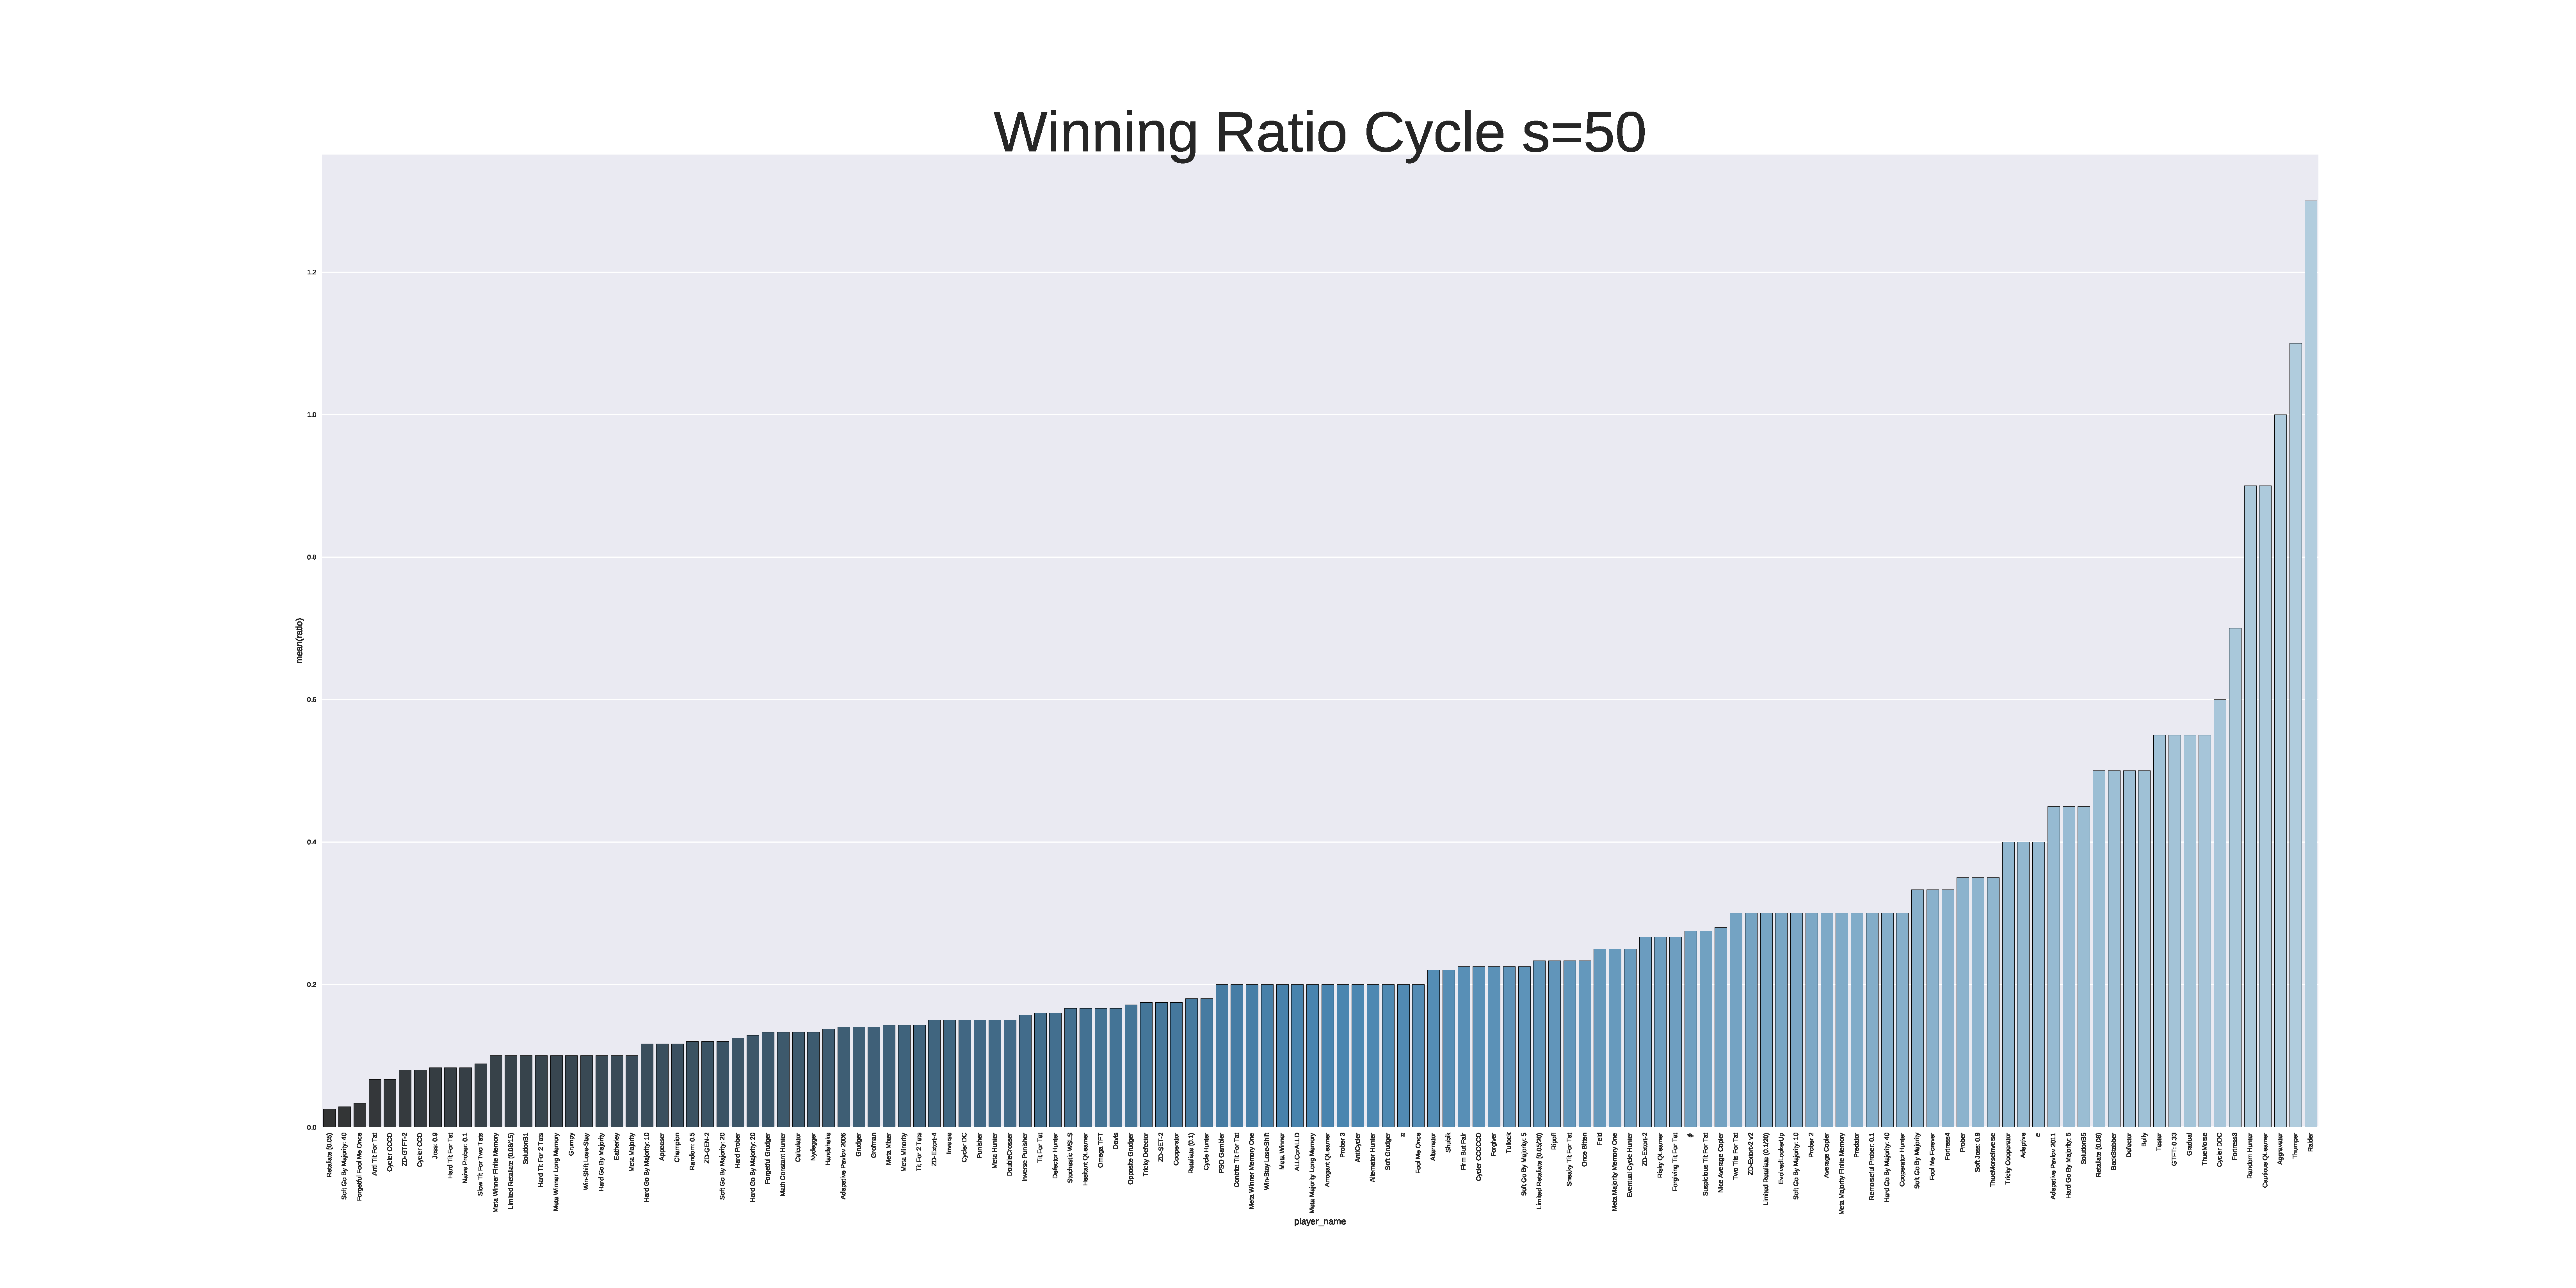
\includegraphics[width=\linewidth]{winners-cycle_fifty.pdf}
    \caption{Winning ration cycle s=50.}
    \end{subfigure}
\hfill
    \begin{subfigure}[t]{1\textwidth}\centering
    \centering
        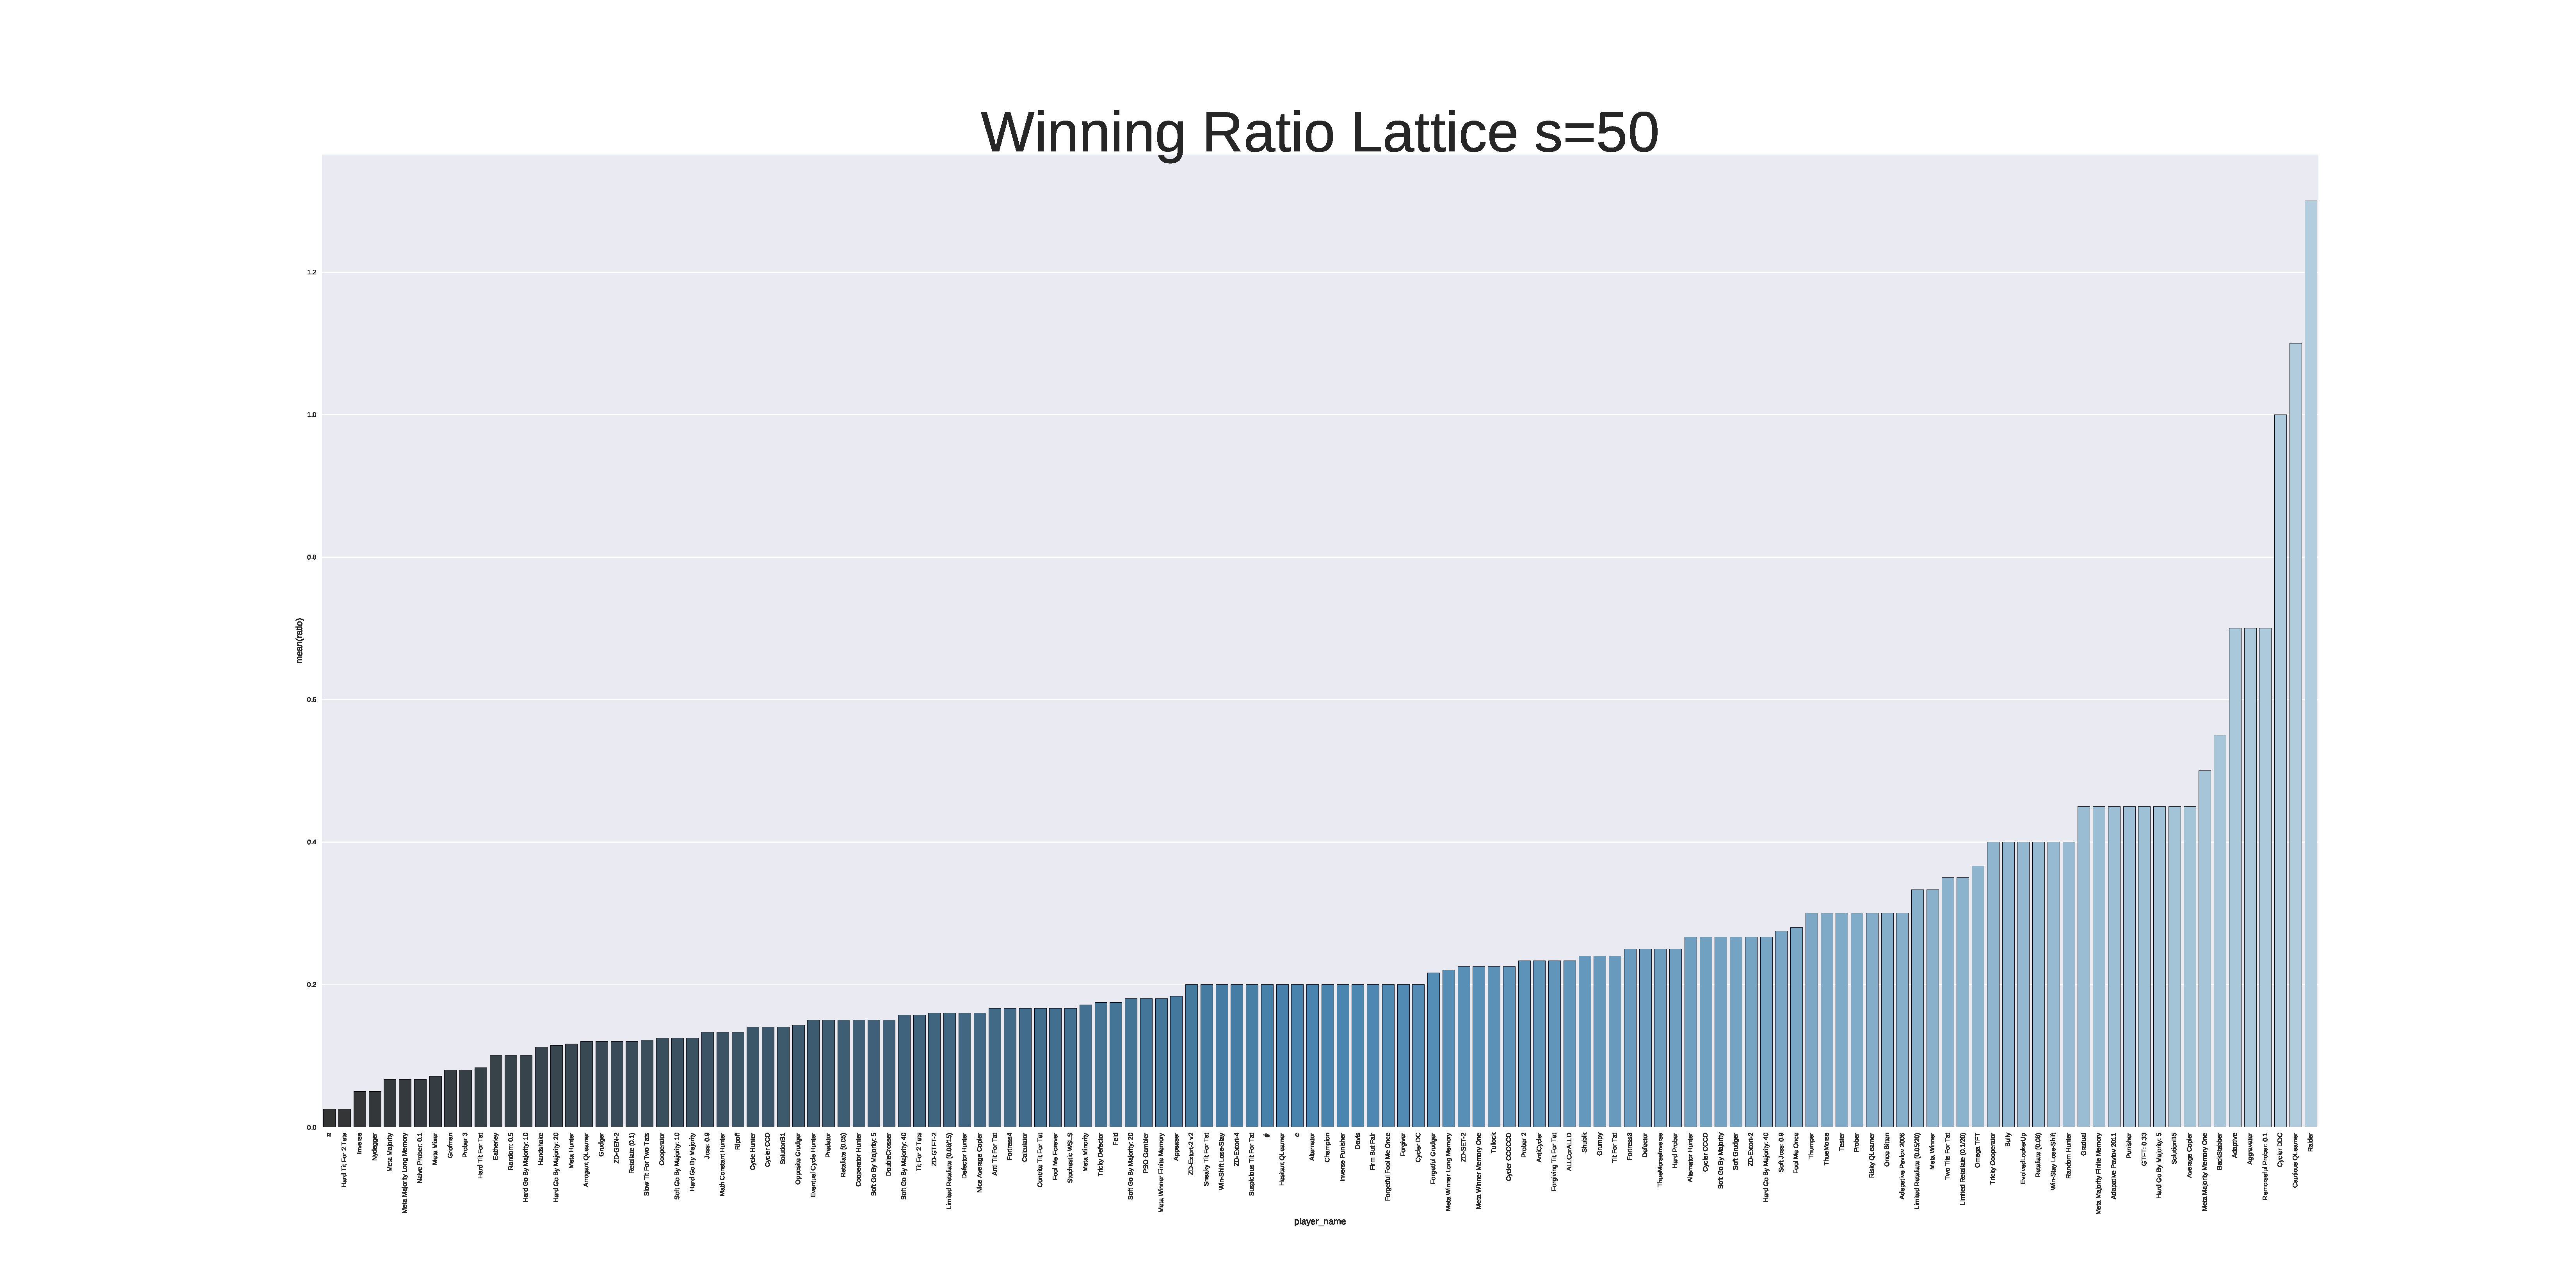
\includegraphics[width=\linewidth]{winners-lattice_fifty.pdf}
    \caption{Winning ration lattice s=50.}
    \end{subfigure}
\hfill
    \begin{subfigure}[t]{1\textwidth}\centering
    \centering
        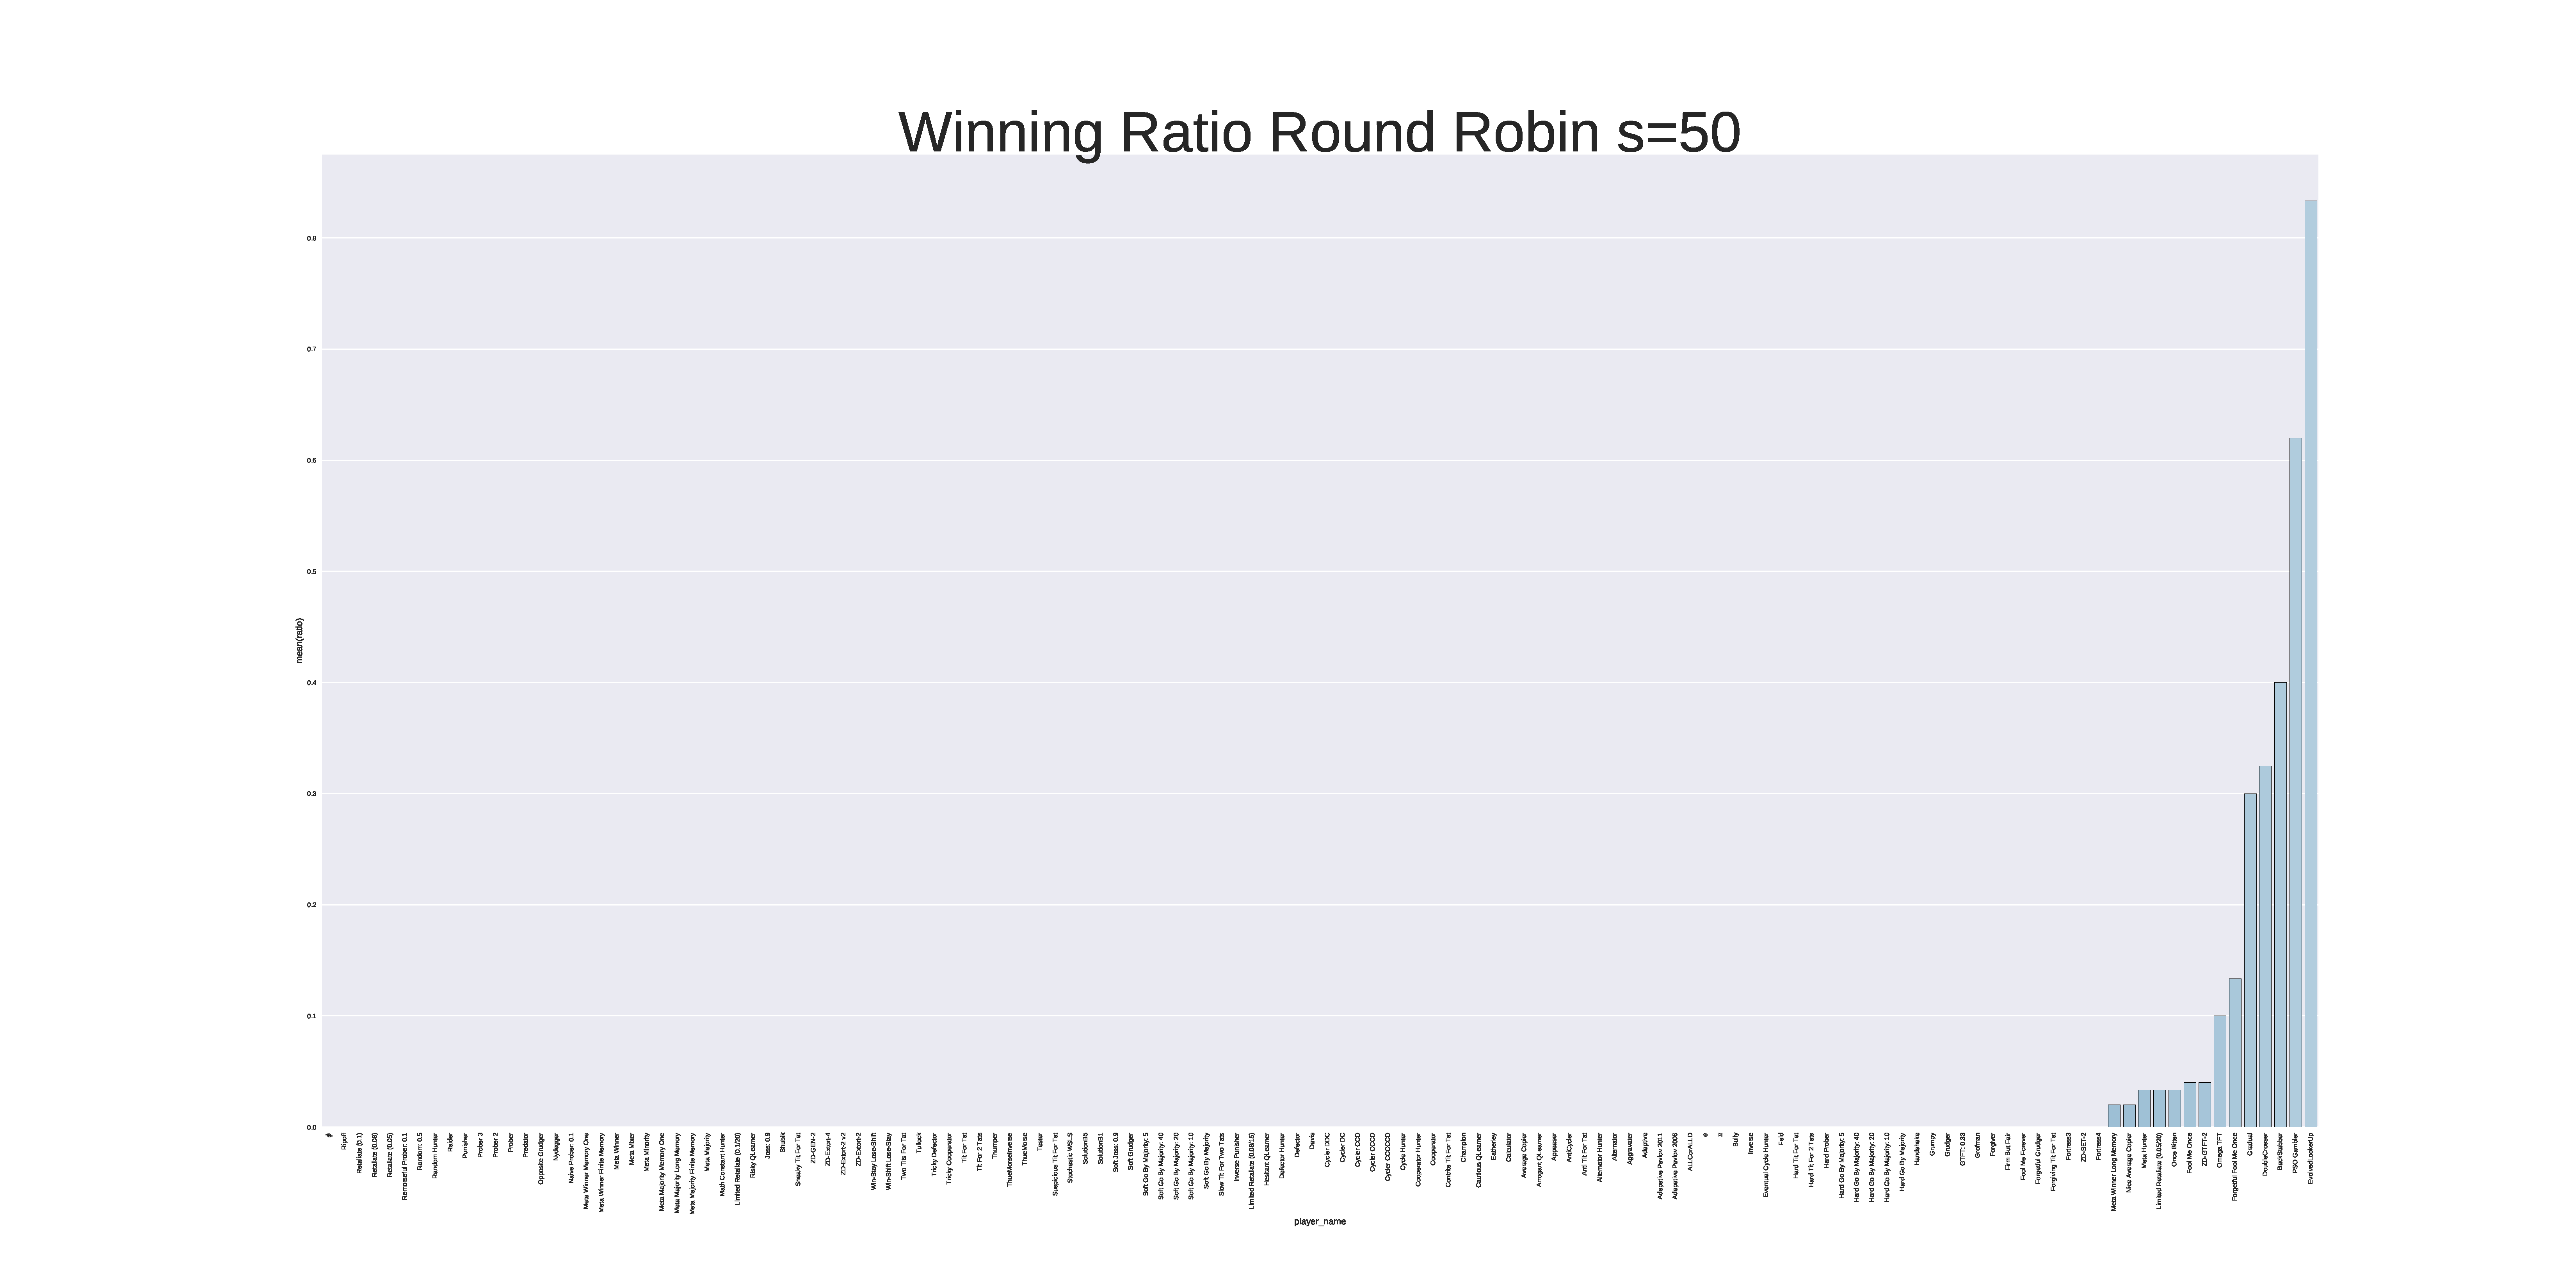
\includegraphics[width=\linewidth]{winners-rr_fifty.pdf}
    \caption{Winning ration round robin s=50.}
    \end{subfigure}
\caption{Winning ratio for all three topologies s=50.}
\label{fig:winning-fifty}
\end{figure}

Now that the winning strategy seem to give us no hind as to how to perform
well in any given random situation we will do further investigation.
% What do you mean? I thought it did? Once we see those line plots it will be
% easier to see...
The winning ratio was plotted against the number of participations of each
strategy and the results are shown in Figures~\ref{fig:winning-ratio-five}
and~\ref{fig:winning-ratio-fifty}. A regression line was added to the scatter plots
to be able to visualize and point out any hidden trend.
% So linear regression can't be applied here as the dependent variable is
% discrete. You want to draw violin plots (one for each group) category of
% participation size (and for other similar plots) and then instead of a
% regression line on the whole data: add a regression line going through the
% median (and clearly state that that's what you're doing) and also report the
% output of an ANOVA (which I expect will show no variance between the groups).

For \(s=5\) we observe that for the topologies lattice and round robin
% No s.
the regression line is flat. Indicating that there is no correlation between the
participations and the winning ratio. Thus, for these topologies strategies
that participated for a different number of tournaments could have achieved the
same winning ratio. In the cycle topology, the graph indicates a positive
correlation. For the cycle,
it could be suggested that that the strategies that were ranked first in these
topology had high
participating rates as well. This seems to apply for only the specific experiment.

On the contrary, for \(s=50\) cycle and lattice show to have a negative
effect between participations and winning ratio. An unexpected results. Thus, playing
less in these experiments could help you achieve a better outcome. This results
could be fixed because of the neighborhoods. For a round robin topology
participation does not seem to have any effect.
% Let's see what Anova and the new regression line say about this.

\begin{figure}[!hbtp]
\centering

    \begin{subfigure}[t]{1\textwidth}
    \centering
        \includegraphics[width=\linewidth]{wining-ratio-cycle_five.pdf}
    \caption{Winning ration against number of participations cycle s=5.}
    \end{subfigure}
\hfill
    \begin{subfigure}[t]{1\textwidth}\centering
    \centering
        \includegraphics[width=\linewidth]{wining-ratio-lattice_five.pdf}
    \caption{Winning ration against number of participations lattice s=5.}
    \end{subfigure}
\hfill
    \begin{subfigure}[t]{1\textwidth}\centering
    \centering
        \includegraphics[width=\linewidth]{wining-ratio-rr_five.pdf}
    \caption{Winning ration against number of participations round robin s=5.}
    \end{subfigure}
\caption{Winning ratio against number of participating in a tournament
         for all three topologies s=5.}
\label{fig:winning-ratio-five}
\end{figure}

\begin{figure}[H]
\centering
    \begin{subfigure}[t]{1\textwidth}
    \centering
        \includegraphics[width=\linewidth]{wining-ratio-cycle_fifty.pdf}
    \caption{Winning ration against number of participations cycle s=50.}
    \end{subfigure}
\hfill
    \begin{subfigure}[t]{1\textwidth}\centering
    \centering
        \includegraphics[width=\linewidth]{wining-ratio-lattice_fifty.pdf}
    \caption{Winning ration against number of participations lattice s=50.}
    \end{subfigure}
\hfill
    \begin{subfigure}[t]{1\textwidth}\centering
    \centering
        \includegraphics[width=\linewidth]{wining-ratio-rr_fifty.pdf}
    \caption{Winning ration against number of participations round robin s=50.}
    \end{subfigure}
\caption{Winning ratio against number of participating in a tournament
             for all three topologies s=50.}
\label{fig:winning-ratio-fifty}
\end{figure}

% Summarise and introduce the next section.

\subsection{Average Scores}

The normalized average score is calculated by dividing the average score per
turn per opponent
of each strategy with their participation counts. Then the average score
is plotted against the strategies. As shown in both
Figures~\ref{fig:average-score-five} and~\ref{fig:average-score-fifty}.

For all six experiments the normalized average score seems to have a lot
of variation. Which indicates each strategy performed differently at given
points of the same experiment. These could be because of the opponent or the
whole neighborhood.

Not many conclusions can be made out of this. The high variation could indicate
that the results are completely random. Unfortunately, this could mean that for
any random situation there does not seem to be a strategy that could
achieve a particularly high score although as described in Section~\ref{?} it is
possible to ensure a good performance.
% Move this till after the plots (no problem if they float)

%Change box plots to violin plots
\begin{figure}[!hbtp]
\centering
    \begin{subfigure}[t]{1\textwidth}
    \centering
        \includegraphics[width=\linewidth]{box-plot-cycle_five.pdf}
    \caption{Normalized average score cycle s=5.}
    \end{subfigure}
\hfill
    \begin{subfigure}[t]{1\textwidth}\centering
    \centering
        \includegraphics[width=\linewidth]{box-plot-lattice_five.pdf}
    \caption{Normalized average score cycle s=5.}
    \end{subfigure}
\hfill
    \begin{subfigure}[t]{1\textwidth}\centering
    \centering
        \includegraphics[width=\linewidth]{box-plot-rr_five.pdf}
    \caption{Normalized average score cycle s=5.}
    \end{subfigure}
    % When you make these figures, include a `bbox_inches='tight'` argument in
    % the save call (it will make sure your legend isn't cut off). Let me know
    % if that doesn't make sense. You might need to do that on a few of these.
\caption{Normalized average score for the three topologies s=5.}
\label{fig:average-score-five}
\end{figure}

\begin{figure}[!htbp]
\centering
    \begin{subfigure}[t]{1\textwidth}
    \centering
        \includegraphics[width=\linewidth]{box-plot-cycle_fifty.pdf}
    \caption{Normalized average score cycle s=50.}
    \end{subfigure}
\hfill
    \begin{subfigure}[t]{1\textwidth}\centering
    \centering
        \includegraphics[width=\linewidth]{box-plot-lattice_fifty.pdf}
    \caption{Normalized average score cycle s=50.}
    \end{subfigure}
\hfill
    \begin{subfigure}[t]{1\textwidth}\centering
    \centering
        \includegraphics[width=\linewidth]{box-plot-rr_fifty.pdf}
    \caption{Normalized average score cycle s=50.}
    \end{subfigure}
\caption{Normalized average score for the three topologies s=50.}
\label{fig:average-score-fifty}
\end{figure}

% average score against participations can be added

\subsection{Regression Analysis}

Finally, a common methodology when investing factors as predictors is building a
regression model. We are building a model wanting to identify any factor that can
explain the winning ratio and  average score of a strategy. The round robin
topology is not included in this subsection analysis as this investigation aims
to understand the effect of network topology. We believe
that in a round robin topology factors like do not have significant effects.
% Fix the we's

The second model using the normalized average score is the following :
% What do you mean by second model?

\begin{equation}\label{regmodel}
\begin{split}
normalized\textrm{ }average\textrm{ }score = degree + average\textrm{ }neighborhood\textrm{ }score + \\
clustering + number\textrm{ }of\textrm{ }participations
% Take a look at:
% http://tex.stackexchange.com/questions/218599/multiline-regression-equation-in-latex
% Fix this (in particular the dependent variables should not be in italics).
\end{split}
\end{equation}

The model was used to each of the experiments for lattice and cycle topologies.
% Do you just mean it was used on the total data set?
The results of models are shown below, Table~\ref{regression} :

\begin{table}[!hbtp]
\centering
\begin{adjustbox}{width=1\textwidth}
\small
\begin{tabular}{@{}|l|l|l|l|l|l|l|l|l|l|l|l|l|@{}}
\toprule
Size & Topology & \multicolumn{2}{l|}{Intercept} & \multicolumn{2}{l|}{degree} & \multicolumn{2}{l|}{average neighborhood score} & \multicolumn{2}{l|}{connectivity} & \multicolumn{2}{l|}{participations} & R-square \\ \midrule
     &          & coef            & p            & coef          & p           & coef                      & p                    & coef             & p              & coef                & p             &          \\ \midrule
s=5  & Cycle    & 0.028           & 0.00         & 0.0559        & 0.00        & -3.763e-06                & 0.043                & 0.0              & NA             & -0.0016             & 0.00          & 0.457    \\ \midrule
     & Lattice  & 0.0064          & 0.00         & 0.0256        & 0.00        & 1.079e-05                 & 0.00                 & 0.0064           & 0.00           & -0.0016             & 0.00          & 0.549    \\ \midrule
s=50 & Cycle    & 0.0025          & 0.00         & 0.0051        & 0.00        & -2.168e-07                & 0.00                 & 0                & NA             & -1.602e-05          & 0.00          & 0.120    \\ \midrule
     & Lattice  & 0.0006          & 0.00         & 0.0024        & 0.00        & 1.033e-06                 & 0.00                 & 0.0003           & 0.00           & -1.601e-05          & 0.00          & 0.216    \\ \bottomrule
\end{tabular}
\end{adjustbox}
\caption{Regression results for model ~\ref{regmodel}}
\label{regression}
\end{table}

In the output we can see that Degree, average neighborhood score and participations
are significant predictors for all the experiments with a \(p\) value less than
an 0.05.
% Less than 0 means negative.
For the cycle topology, average neighborhood score and participations have negative
coefficients. For example a decrease in participations by one would increase
the average score by 0.0016. Degree on the other hand has a positive coefficient
and connectivity has no effect at all. Furthermore the model for \(s=5\) has
% No s (find any that I've missed)
a R-square value of 0.457, thus it only explains 0.4 variation of the data which is
quite low. For \(s=50\) it is even lower at only 0.12.

Finally, for the lattice topology only participations have a negative coefficients.
Thus the only factor with a reverse influence on average score in the lattice topology.
Connectivity is a significant predictor as well with a coefficient 0.0064 and
0.0003 respectively. Though the R-square value is still  small,
with a value 0.547 and 0.216 respectively.
Even if there are predictors with a significant \(p\) value, the overall
performance of the model is moderate.

% Can you include a 1 or 2 sentence summary that breaks down the main findings
% of this regression model? Say you walked up to some random person in the
% street and they wanted to know: what would you tell them?

%couldnt get winning ration in data frame
% This is fixed now yes?

\section{Summary}

In this section we will make a summary of all the previous analysis that was made
in~\ref{sub:effects} and list further research that could be performed.

From the analysis that was performed in~\ref{sub:winning-ratio}, the wining ratio
for each strategy for all 6 experiments indicated the following :

\begin{itemize}
  \item For the cycle topology of \(s=5\) ZD-GEN-2 had the highest winning ratio
      % No s
        and for the lattice BackStabber and Meta Majority Memory one
  \item For round robin s=50, most of the strategies finished the experiment
        with winning ratio of zero.
  \item Raider seem to have successful performance in both the lattice and cycle \(s=50\)
        and in the round robin \(s=5\).
\end{itemize}

An attempt to find any significant reason as to why these strategies outperform
the rest gave the findings below:

\begin{itemize}
  \item Participating rate has a negative effect on the winning ratio for \(s=50\)
        in lattice and cycle topology and a positive in cycle for \(s=5\)
  \item There is high variation is the average score of each strategy for all
        experiments
  \item A regression model for the normalized average score did not return any
        significant results.
\end{itemize}

Even so, Raider stand out we could not produce any valid facts as to why this
was not random and the Raider base on a number of reasons performed so well.
Numerous actions could solve this. Actions that will be taking into consideration
in the experiments to follow. Firstly, the network topologies used have been
simple examples of graph, thus more sophisticated graphs will be used
with different range of neighborhood sizes. Additionally, having a measure of
comparing strategies will be useful. Thus, we will keep track of the cooperating
rate of the strategies in the future.
% The English isn't great in this paragraph. You should take a look at what
% these strategies (RAider, etc) do, and comment on that.

% Final comment should be about what will be in the next chapter.
